\chapter{Interfaccia}\label{ch:chapter4}

\section{Introduzione}
Nonostante il nucleo principale di questa tesi fosse costruire il modello di ottimizzazione per la programmazione dei turni, è stata anche creata un'interfaccia base per mostrare un utilizzo vero e proprio del programma.
Per far questo è stato utilizzato Django, framework per Python, che ha permesso di sviluppare il lato server dell'applicazione \cite{ref:Django}.

Nella schermata principale è possibile visualizzare gli orari presenti nel database o crearne uno nuovo da zero. Selezionando un orario specifico è possibile, inoltre, visualizzarne i dettagli, come il numero di settimane e il numero di infermieri di cui si vuole gestire la pianificazione dei turni.
Inoltre, dato l'orario, per ogni tipologia di contratto presente è possibile assegnare differenti valori ad alcuni paramatri tra cui il numero minimo e massimo di giorni lavorativi/liberi consecutivi che un infermiere può svolgere.
È possibile inoltre specificare i dettagli di ogni infermiere, con le relative richieste che ognuno di essi può presentare. Infine, nella schermata finale, viene riportato l'output del programma.

\section{Orari}
\begin{figure}[H]
\begin{center}
  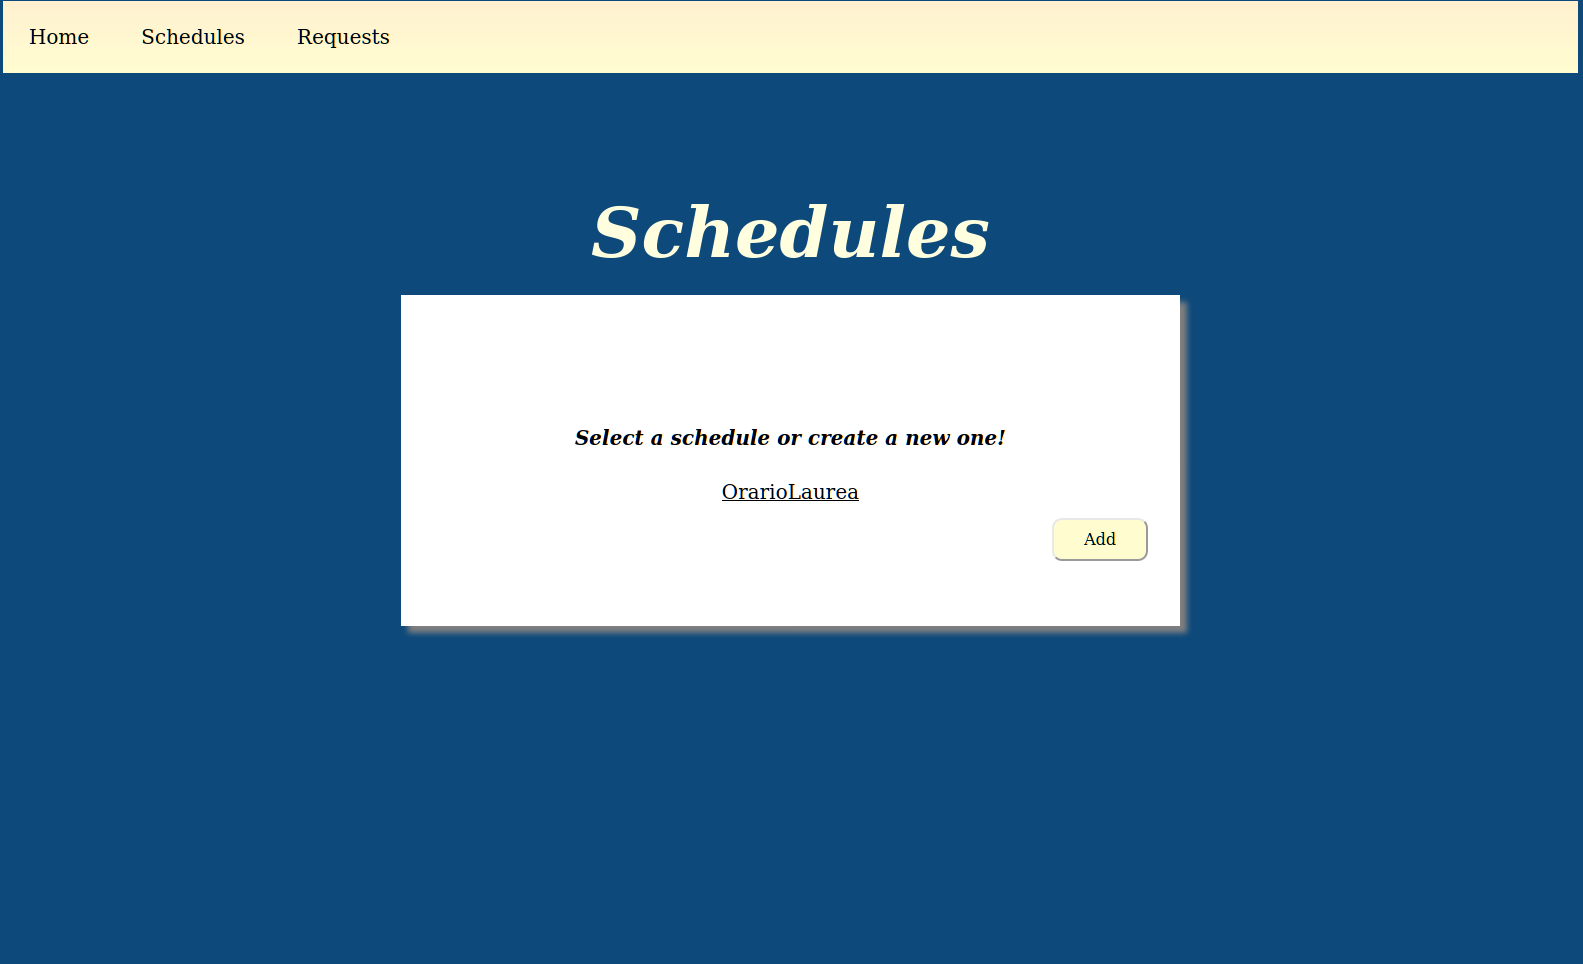
\includegraphics[scale=0.20]{img/Schermate/S1.png}\\
  \caption{Schermata Orari}
\end{center}
\end{figure}

\section{Dettagli Orario}
\begin{figure}[H]
\begin{center}
  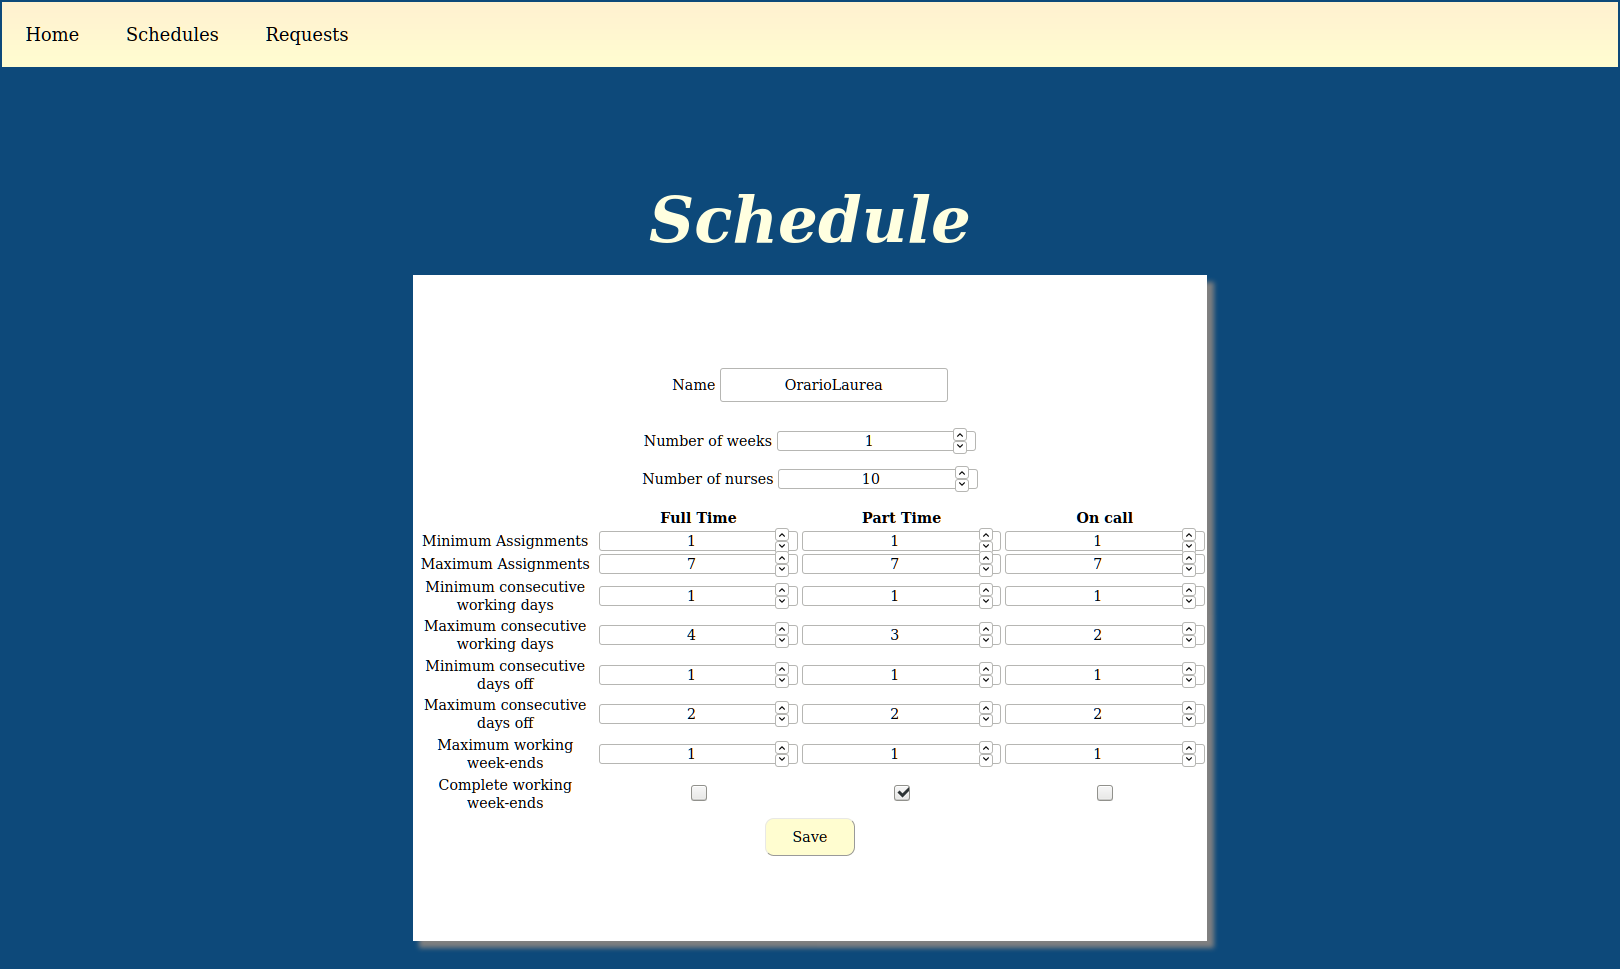
\includegraphics[scale=0.20]{img/Schermate/S2.png}\\
  \caption{Schermata dettagli Orario}
\end{center}
\end{figure}

\section{Dettagli Infermiere}
\begin{figure}[H]
\begin{center}
  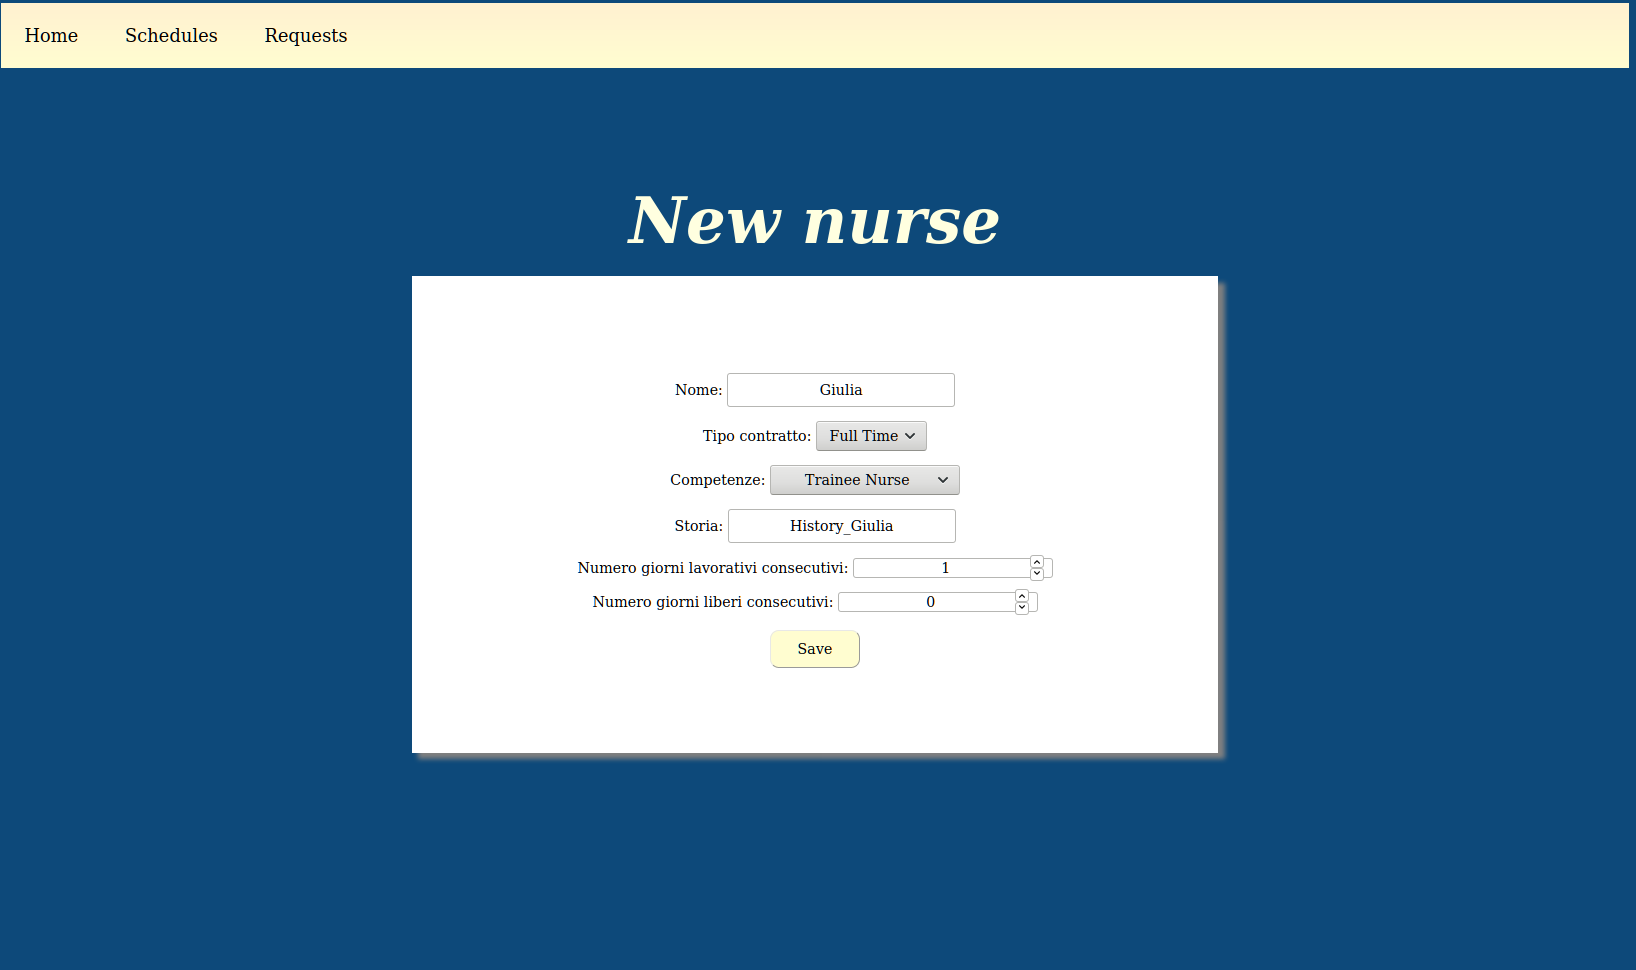
\includegraphics[scale=0.20]{img/Schermate/S5.png}\\
  \caption{Schermata dettagli Infermiere}
\end{center}
\end{figure}

\section{Richiesta Infermiere}
\begin{figure}[H]
\begin{center}
  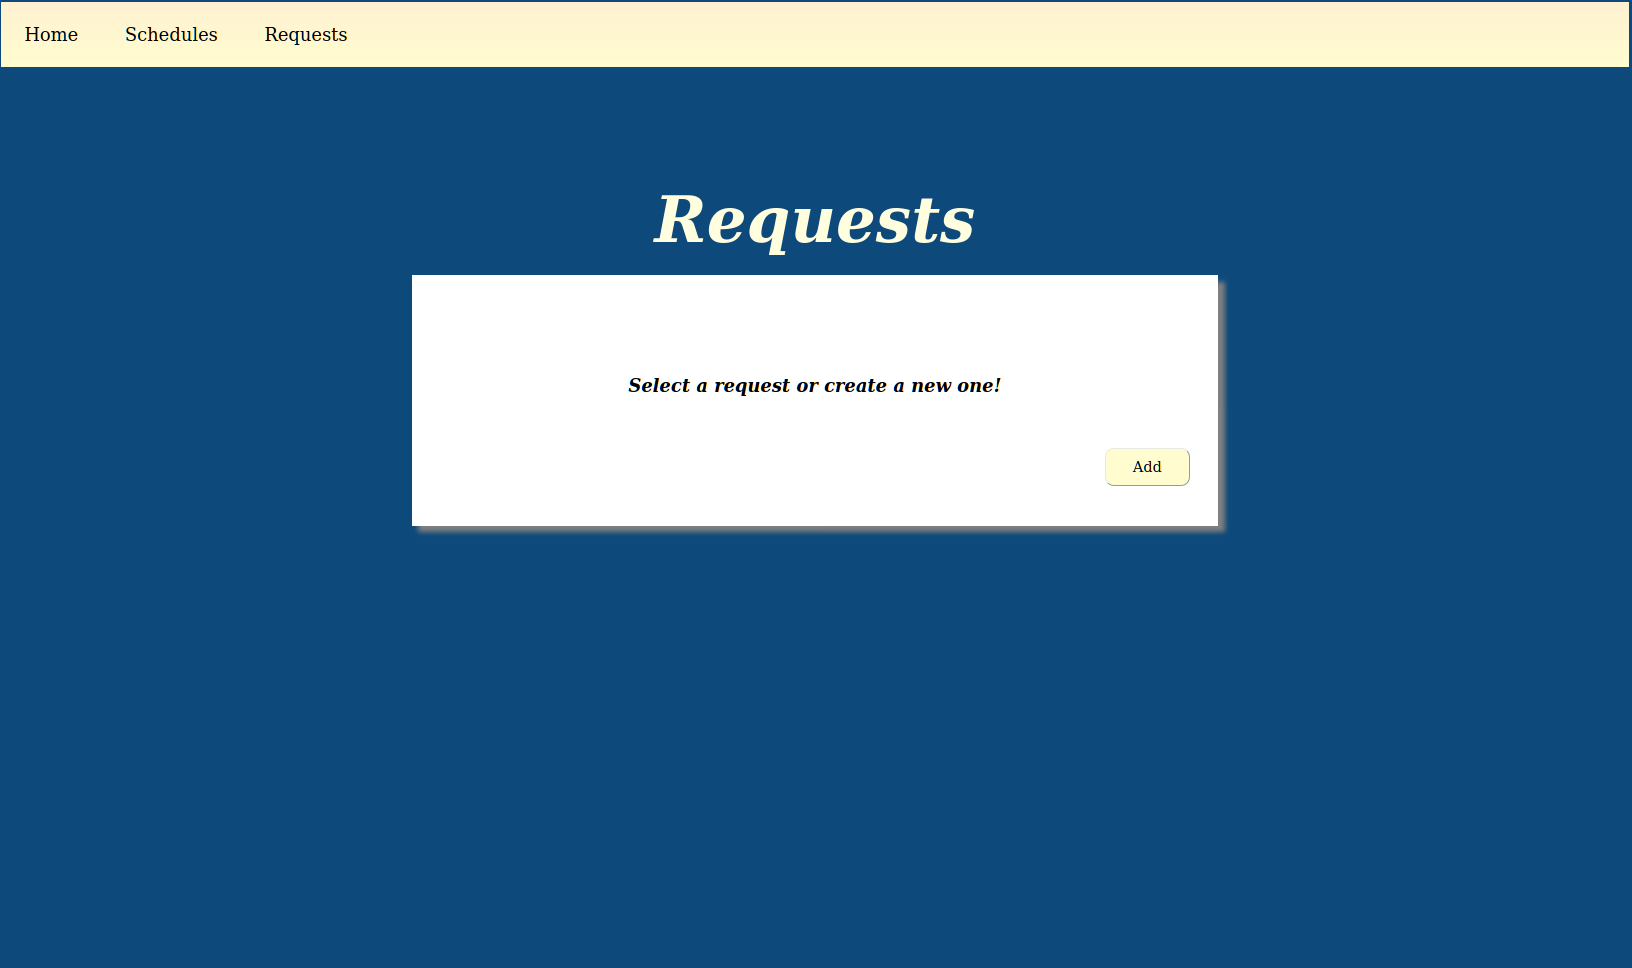
\includegraphics[scale=0.20]{img/Schermate/S3.png}\\
  \caption{Schermata Richieste}
\end{center}
\end{figure}

\begin{figure}[H]
\begin{center}
  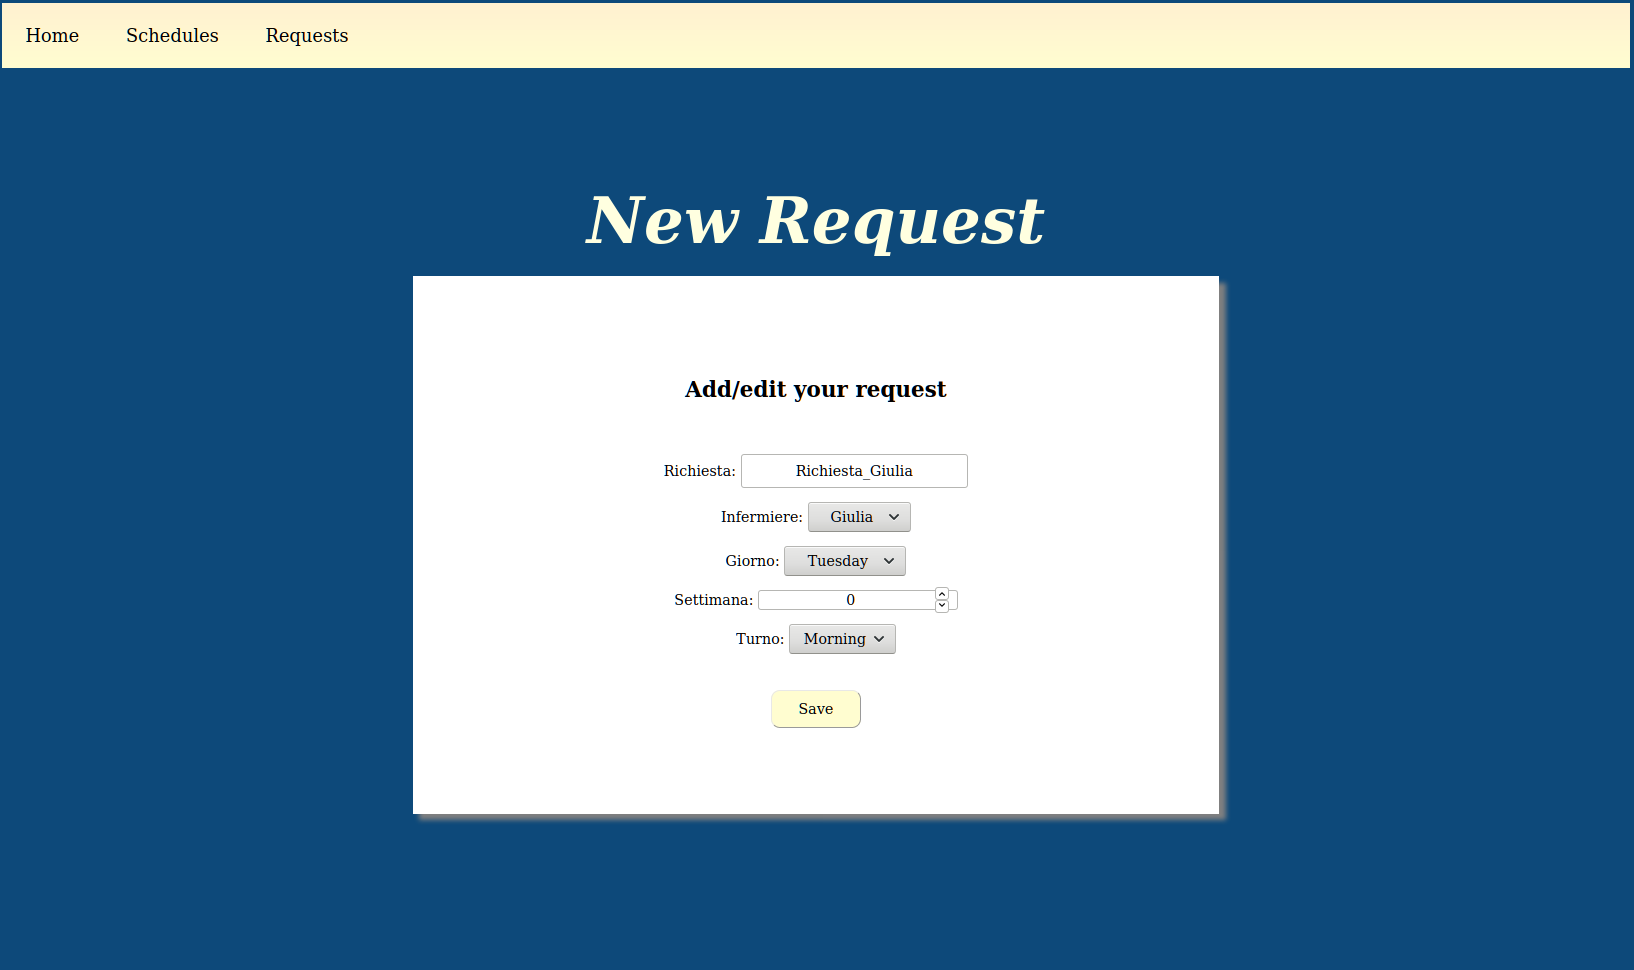
\includegraphics[scale=0.20]{img/Schermate/S4.png}\\
  \caption{Schermata richiesta Infermiere}
\end{center}
\end{figure}

\section{Risultato}
\begin{figure}[H]
\begin{center}
  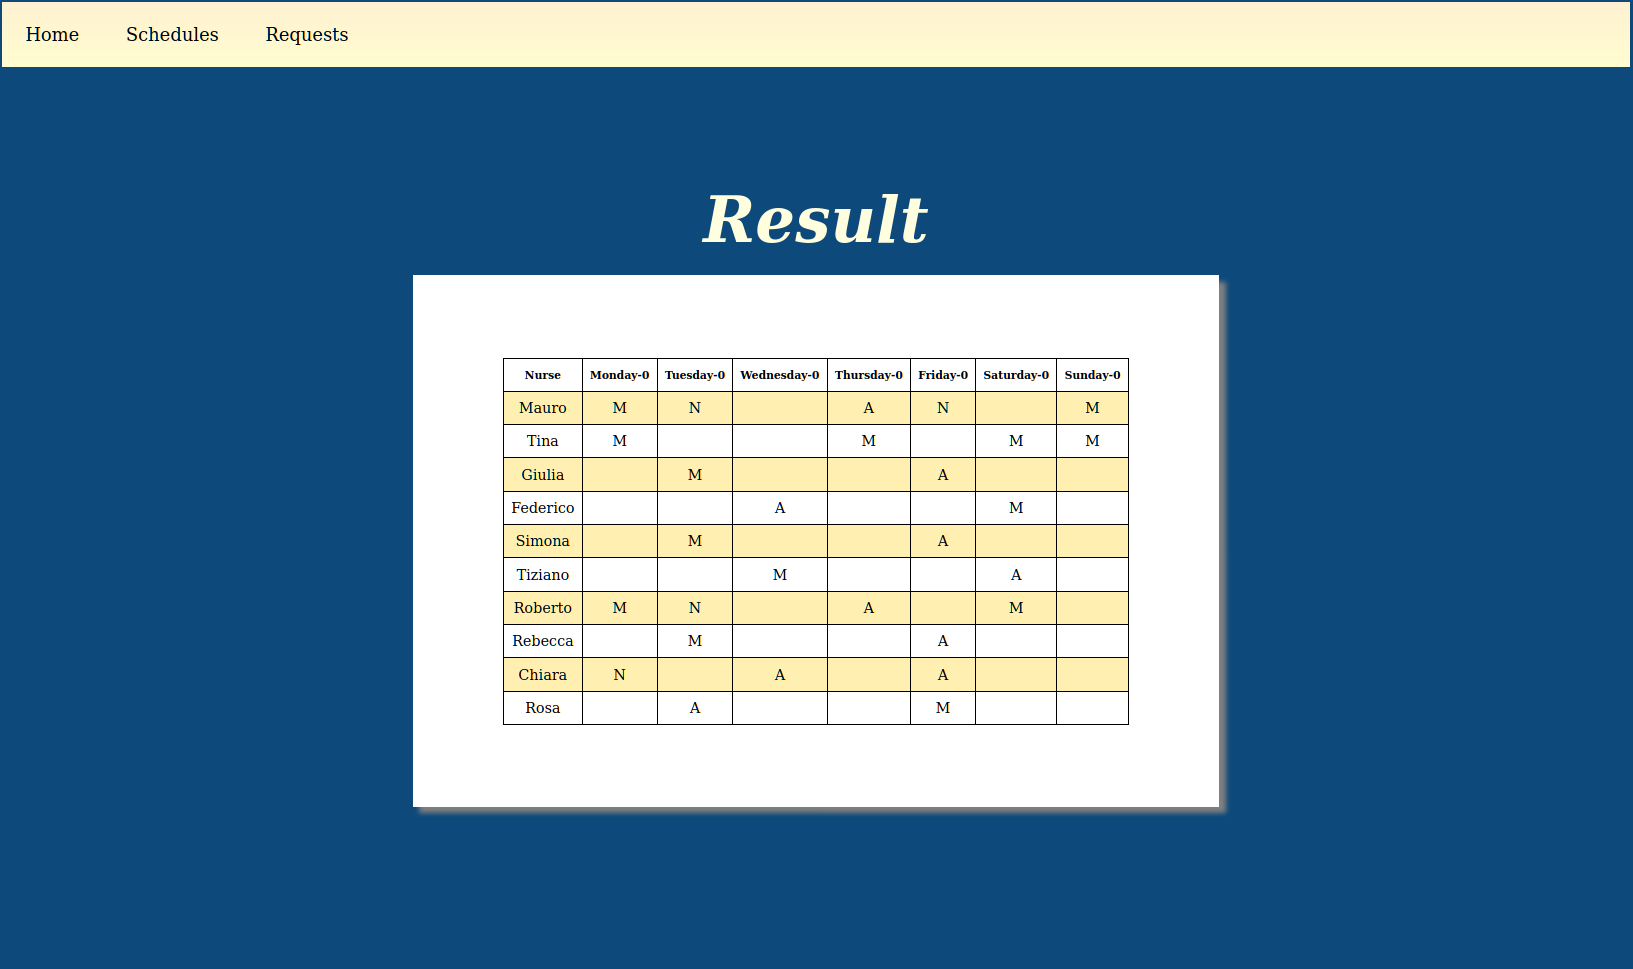
\includegraphics[scale=0.20]{img/Schermate/Result.png}\\
  \caption{Schermata Risultato}
\end{center}
\end{figure}
